


At the core of the language of modeling is the notation that uses the
tilde character (\code{~}) to identify the response variable and the
explanatory variables.  This notation is incorporated into many of
operators that you will use.  

To illustrate the computer commands for modeling and graphically displaying
relationships between variables, use the utilities data 
set:\datasetUtilities. 
\begin{Schunk}
\begin{Sinput}
> require(mosaic)
> utils = fetchData("utilities.csv")
\end{Sinput}
\end{Schunk}
Some of the following examples make particular use of these variables 
\begin{itemize}
\item \VN{ccf} --- the natural gas usage in cubic feet during the
  billing period.
\item \VN{month} --- the month coded as 1 to 12 for January to December.
\item \VN{temp} --- the average temperature during the billing period.
\end{itemize}

Another illustrative example uses
Current Population Survey wage data:\datasetCPS
\begin{Schunk}
\begin{Sinput}
> cps = fetchData("cps.csv")
\end{Sinput}
\end{Schunk}
and focuses on the variables \VN{wage}, \VN{sex}, and \VN{sector}.

\subsection{Bi-variate Plots}

\index{C}{graphics!two-variable}
\index{C}{scatter plot}
\index{P}{scatter plots, making}
\index{P}{Plotting \& Graphics!xyplot@\texttt{xyplot}}
\index{P}{xyplot@\texttt{xyplot}}

The basic idea of a bi-variate (two variable) plot is to examine one
variable as it relates to another.  The conventional format is to plot
the response variable on the vertical axis and an explanatory variable
on the horizontal axis.  

\subsubsection{Quantitative Explanatory Variable}

When the explanatory variable is quantitative, a scatter-plot is an
appropriate graphical format.  In the scatter plot, each case is a
single point.

The basic computer operator for making scatter plots is \function{xyplot}:

\begin{Schunk}
\begin{Sinput}
> xyplot(ccf ~ temp, data=utils)
\end{Sinput}
\end{Schunk}
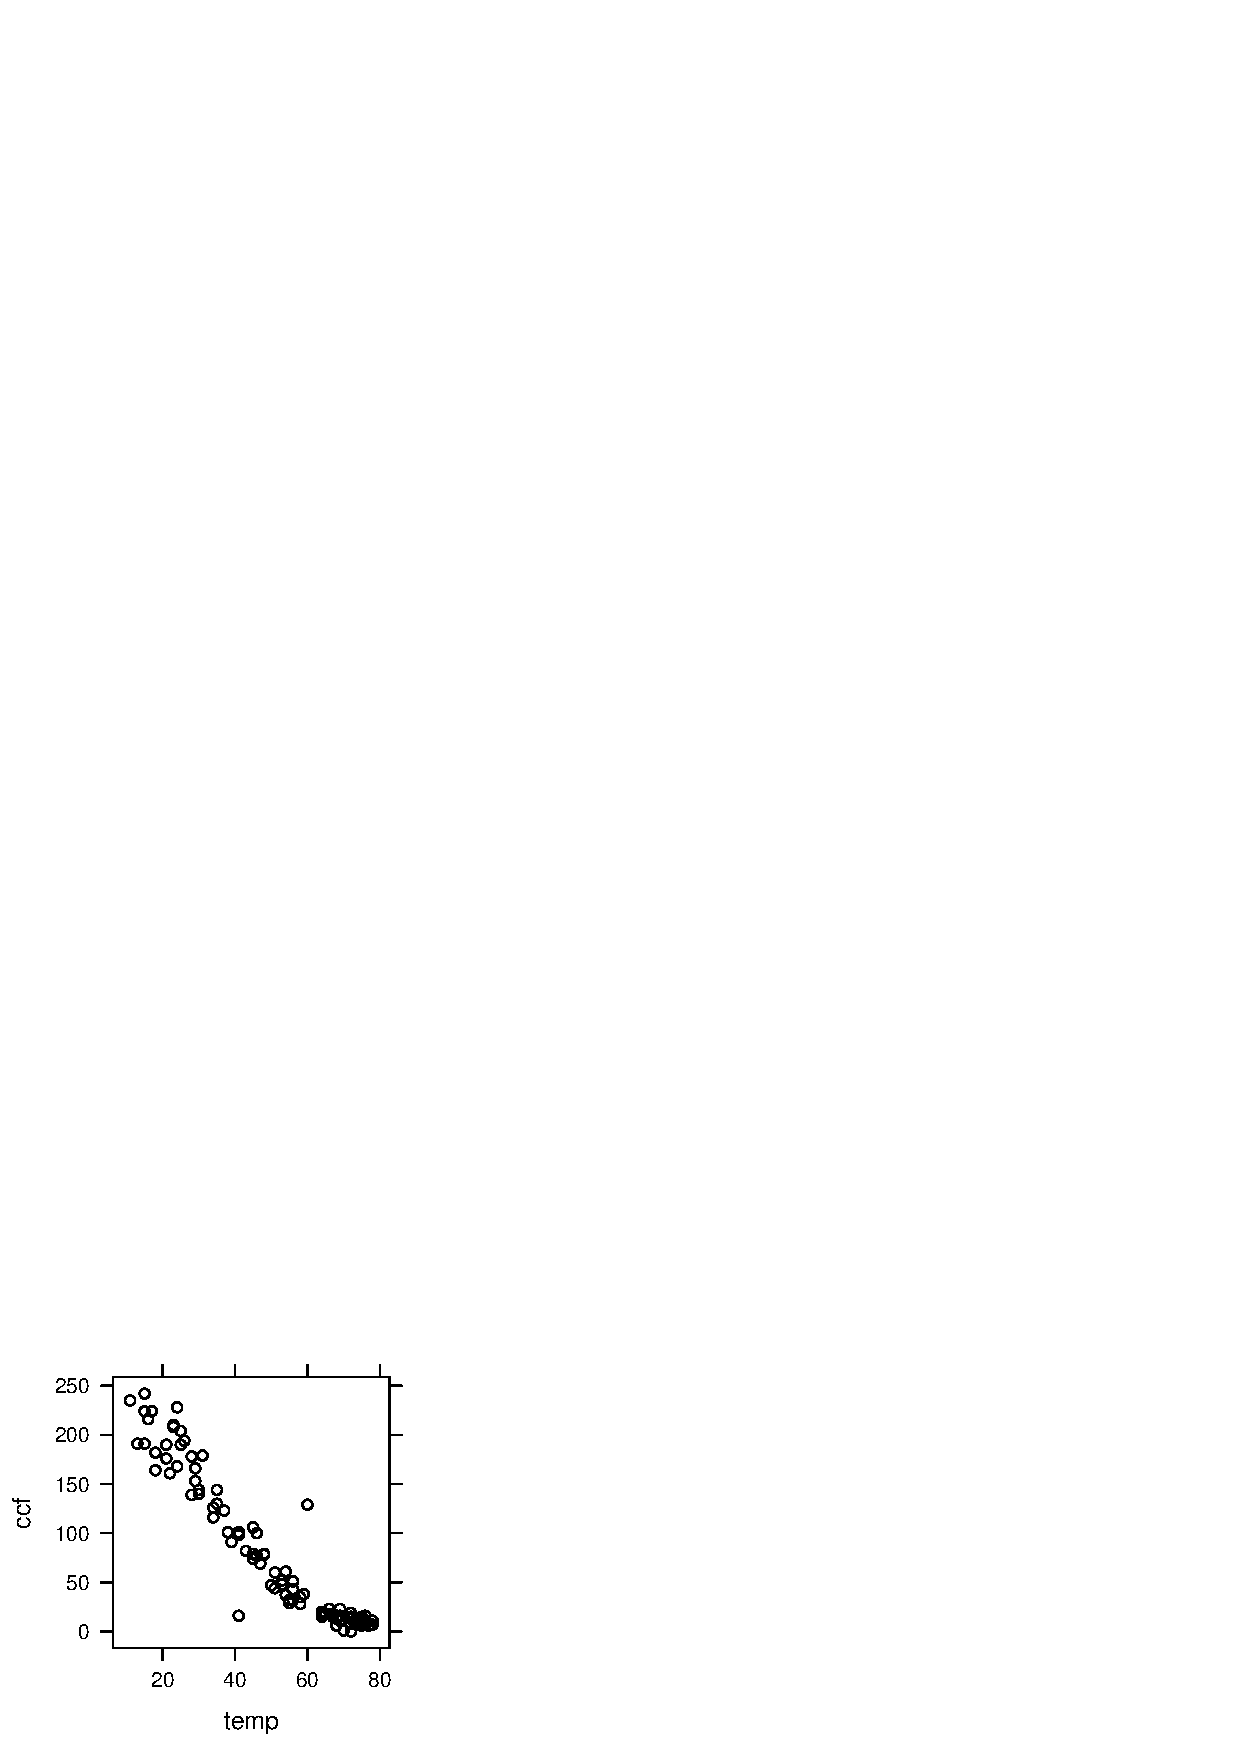
\includegraphics{Figures/language-utils-scatter}

The first argument is a model formula written using the
``\model{}{}'' modeling notation. This formula,
\model{\VN{ccf}}{\VN{temp}} is pronounced ``ccf versus temperature.''

%\noindent\graphicsfile[width=2.5in]{scatter1.pdf}

In order to keep the model notation concise, the model formula has
left out the name of the data frame to which the variables belong.
Instead, the frame is specified in the \code{data} argument.  Since
\code{data} has been set to be \code{utils}, the formula 
\code{ccf ~  temp} is effectively 
translated to \code{utils$ccf ~ utils$temp}. 
\index{P}{data@\texttt{data=} in \texttt{lm}}
\index{P}{Data!data@\texttt{data=} in \texttt{lm}}
\index{P}{Modeling!data@\texttt{data=} in \texttt{lm}}


You can specify the labels by hand, if you like.  For example, 
\begin{Schunk}
\begin{Sinput}
> xyplot( ccf ~ temp, data=utils, 
      xlab="Temperature (deg F)",
      ylab="Natural Gas Usage (ccf)")
\end{Sinput}
\end{Schunk}
\index{C}{graphics!axis labels}
\index{C}{axis (in graphics)!labels}
\index{P}{xlab@\texttt{xlab=} for axis label}
\index{P}{ylab@\texttt{ylab=} for axis label}
\index{P}{Plotting \& Graphics!xlab@\texttt{xlab=} \& \texttt{ylab=}}


\subsubsection{Categorical Explanatory Variable}

When the explanatory variable is categorical, an appropriate format of
display is the box-and-whiskers plot, made with the \code{bwplot}
operator.   Here, for example, is the
\VN{wage} versus \VN{sex} from the Current Population Survey:
\index{P}{bwplot@\texttt{bwplot}}
\index{P}{Plotting \& Graphics!bwplot@\texttt{bwplot}}
\index{C}{box plot!drawing}
\begin{Schunk}
\begin{Sinput}
> bwplot( wage ~ sex, data=cps)
\end{Sinput}
\end{Schunk}
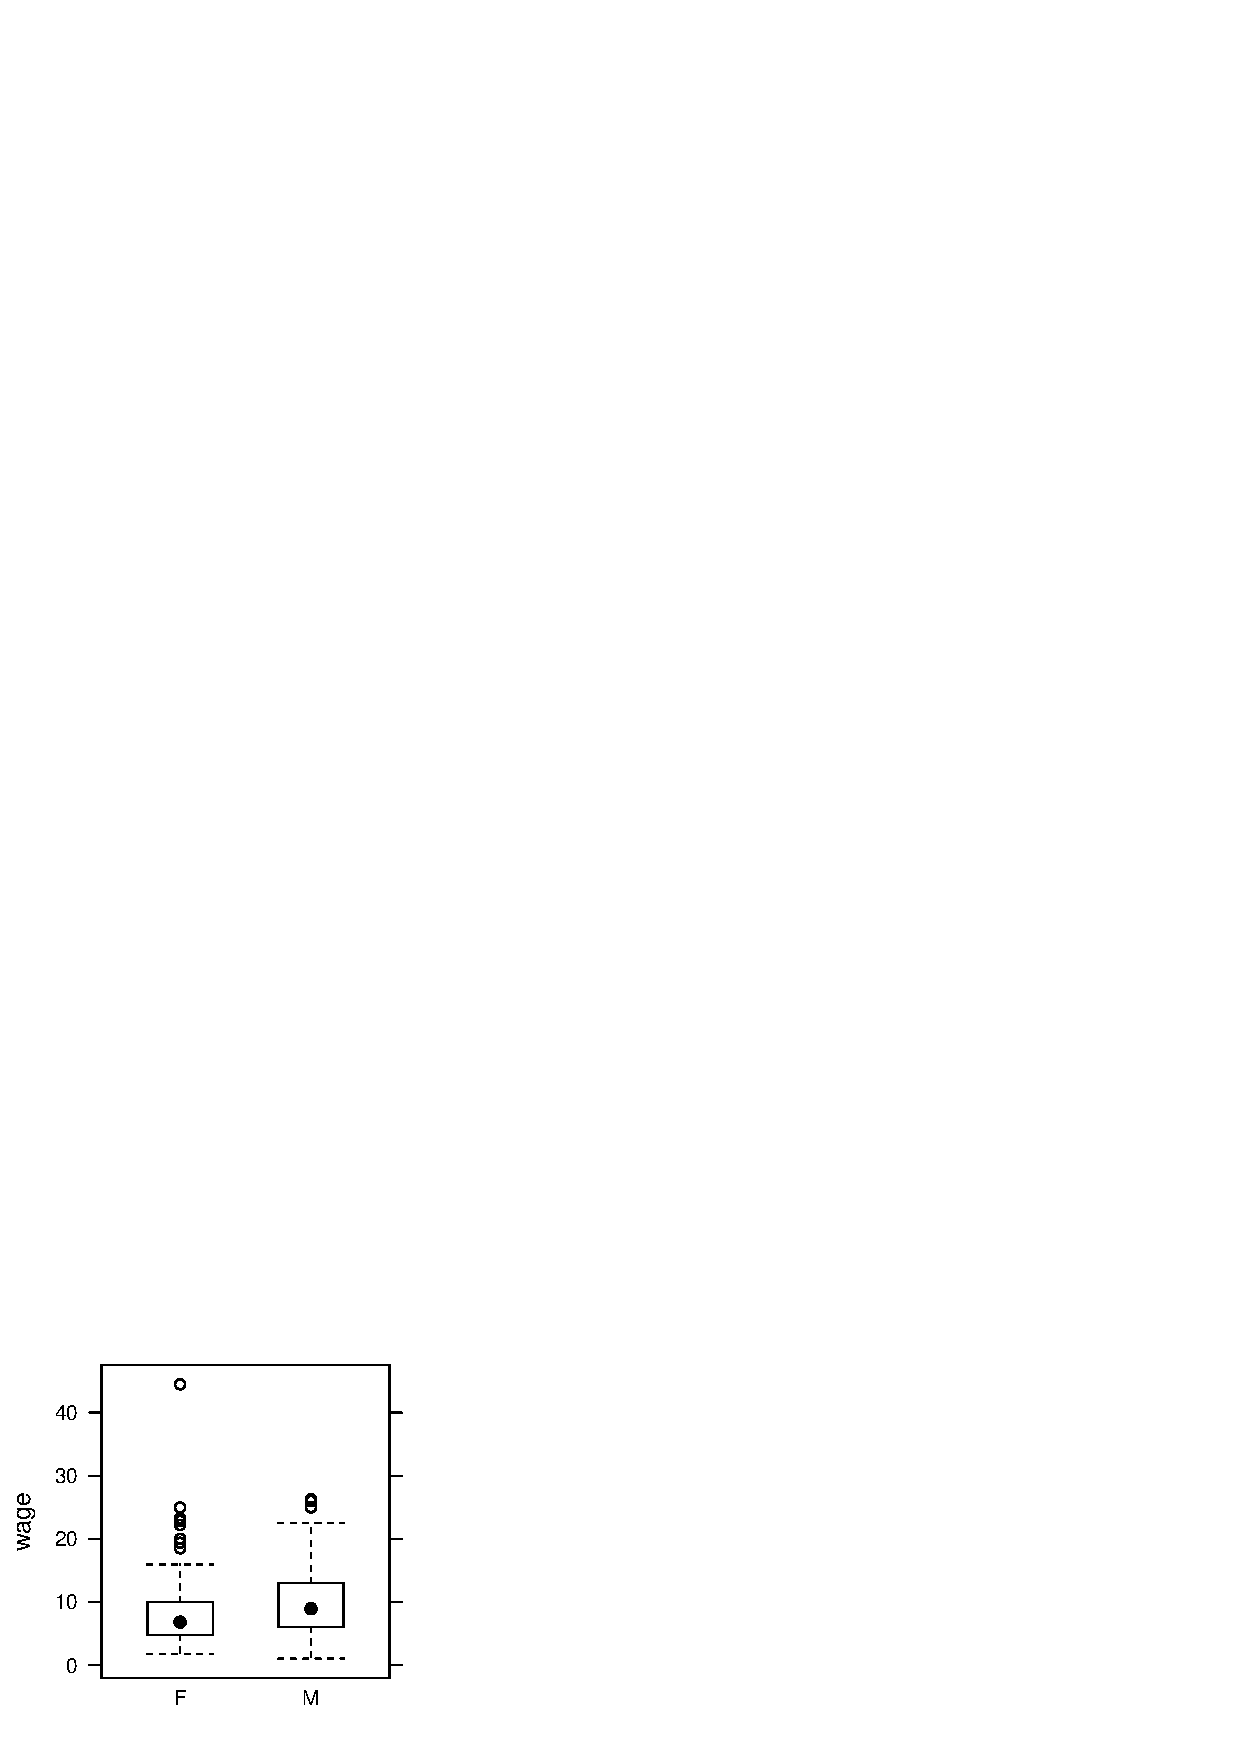
\includegraphics{Figures/language-box1}
% \noindent\graphicsfile[width=2.5in]{box1.pdf}

\index{P}{Plotting \& Graphics!axis limits}
\index{C}{graphics!axis limits}
\index{C}{axis (in graphics)! limits in graphics}
\index{P}{xlim@\texttt{xlim=} for axis limits}
\index{P}{ylim@\texttt{ylim=} for axis limits}

Notice that the outliers are setting the overall vertical scale for
the graph and obscuring the detail at typical wage levels.  You can
use the \code{ylim} argument to set the scale of the y-axis however
you want. For example:

\begin{Schunk}
\begin{Sinput}
> bwplot(wage~sector, data=cps, ylim=c(0,30) )
\end{Sinput}
\end{Schunk}

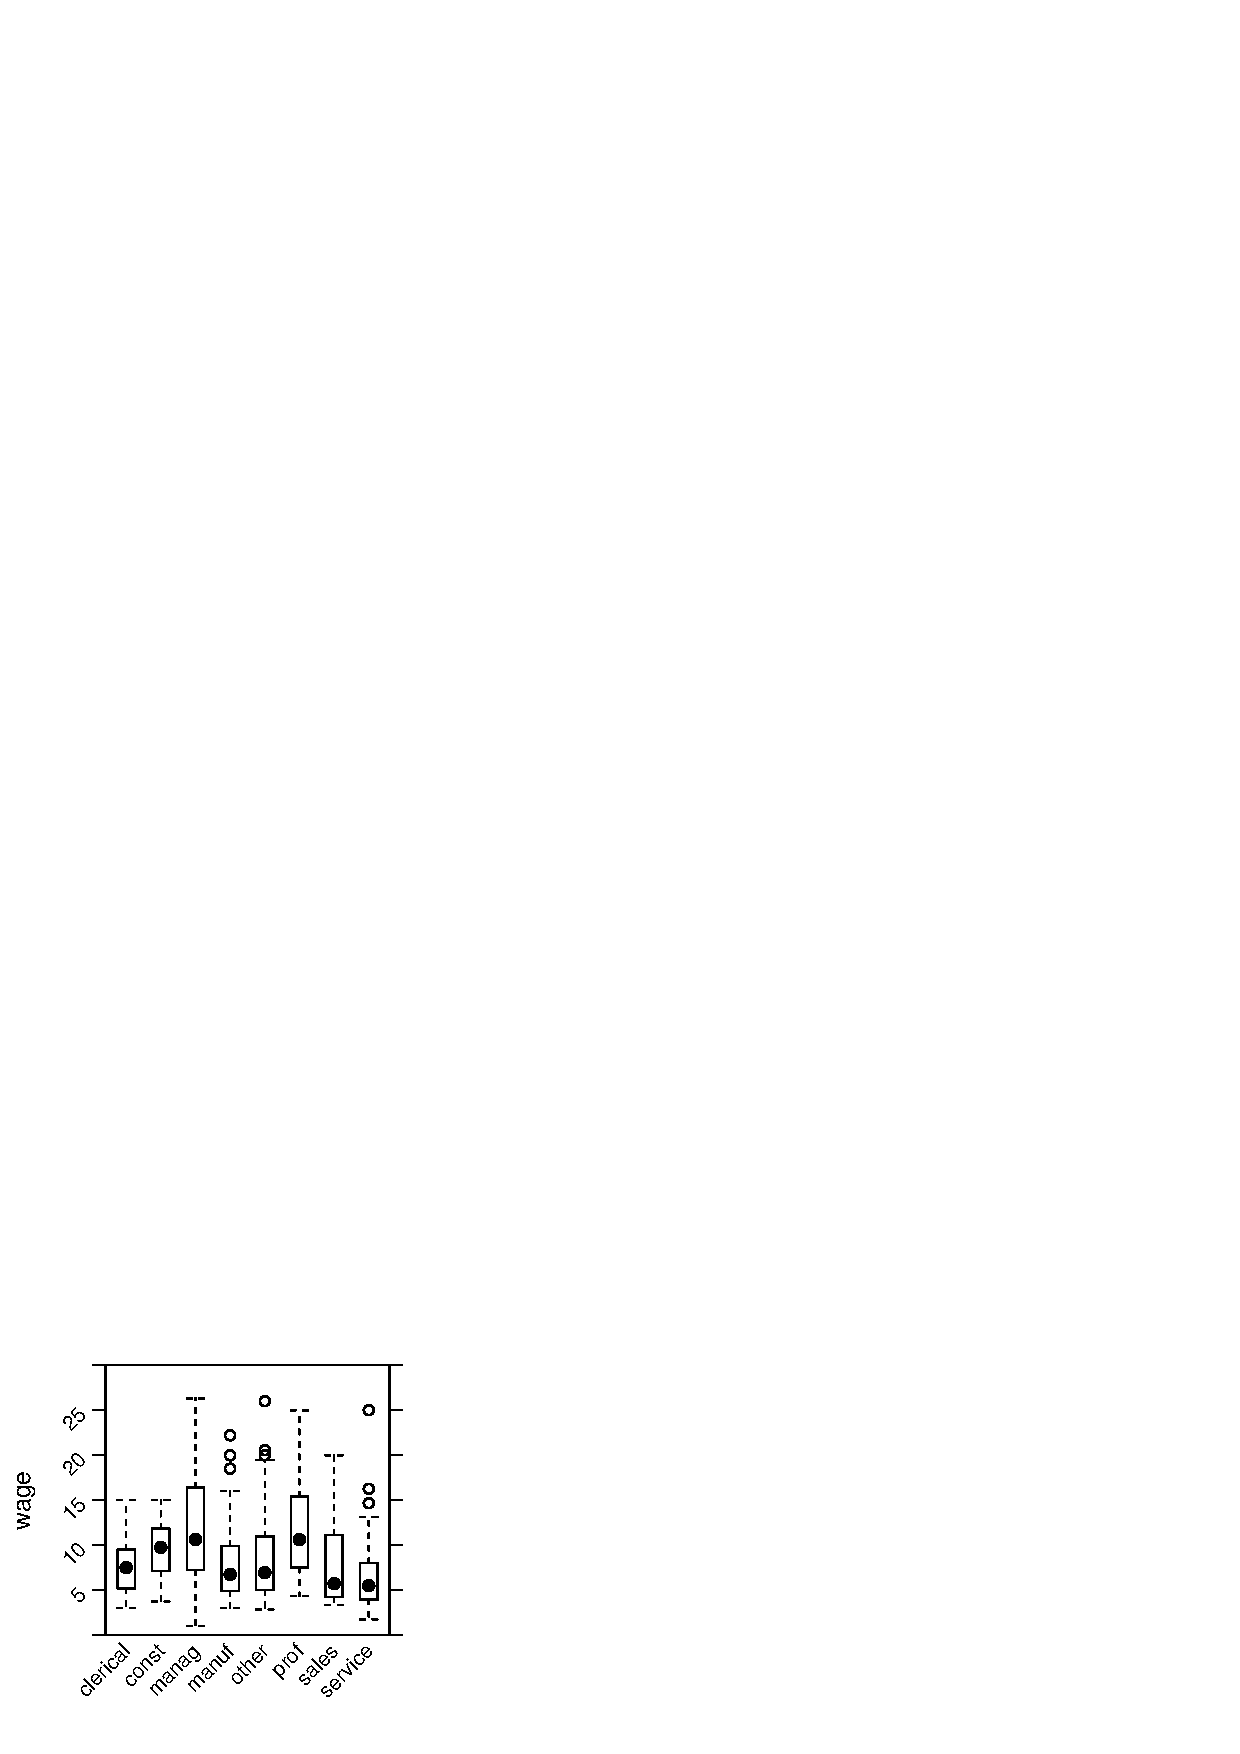
\includegraphics{Figures/language-box3}
%\noindent\graphicsfile[width=2.5in]{box3.pdf}

You can also make side-by-side density plots which show more detail than the
box-and-whisker plots.  For instance:
\index{P}{densityplot@\texttt{densityplot}}
\index{P}{Plotting \& Graphics!densityplot@\texttt{densityplot}}
\index{P}{key in graphics, \texttt{auto.key=}}
\index{P}{auto.key@\texttt{auto.key=}}
\index{C}{Plotting \& Graphics!adding a key}
\begin{Schunk}
\begin{Sinput}
> densityplot( ~ wage, groups=sex, data=cps, auto.key=TRUE )
\end{Sinput}
\end{Schunk}
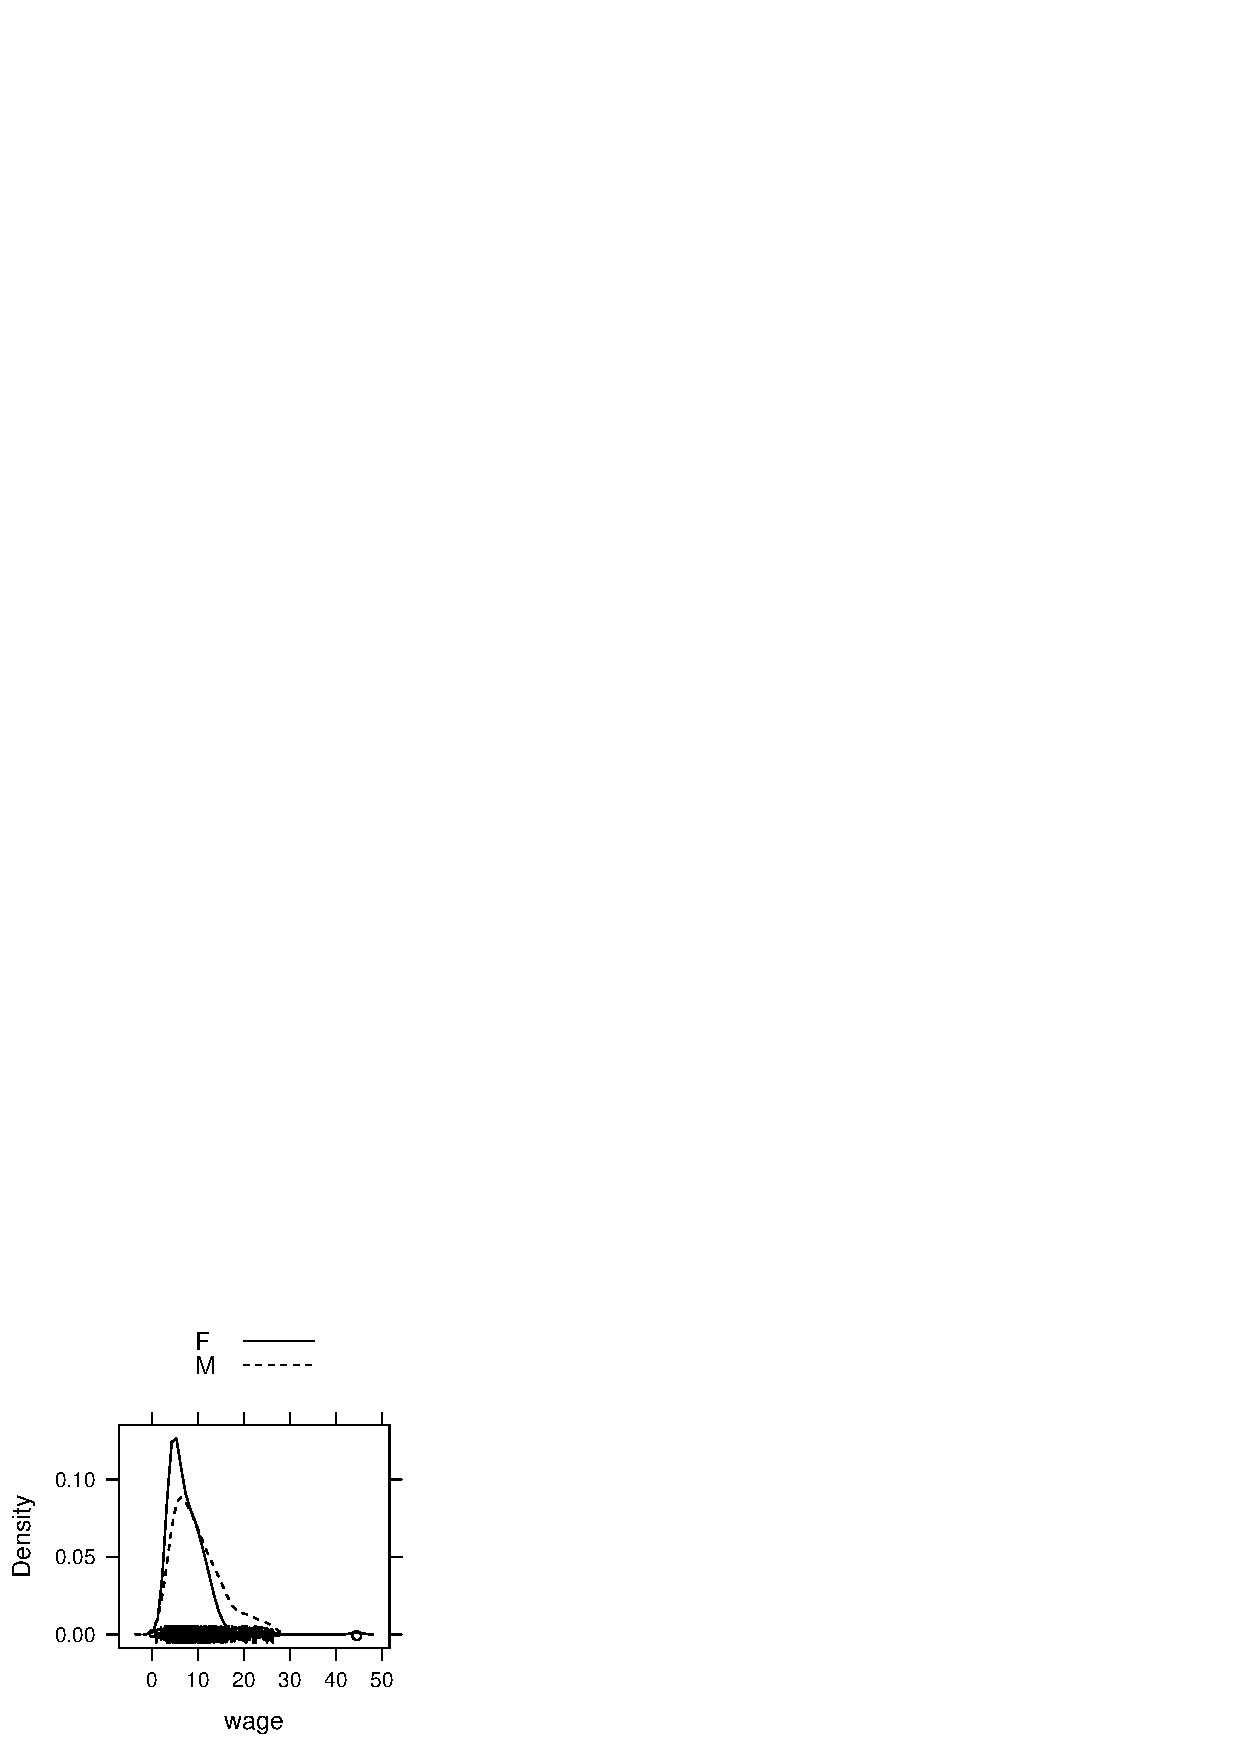
\includegraphics{Figures/language-side-by-side-density}
%\noindent \graphicsfile[width=2.5in]{side-by-side-density.pdf}

\noindent 
It seems a bit odd to have the notation \code{~ wage} --- nothing is in the role of the response variable.  This idiosyncratic notation perhaps is meant to
reflect that \VN{wage} is on the horizontal axis.

\subsubsection{Multiple Explanatory Variables}

\index{C}{graphics!multiple variables}


The two-dimensional nature of paper or the computer screen lends
itself well to displaying two variables: a response versus a single
explanatory variable.  Sometimes it is important to be able to add an
additional explanatory variable.  The graphics system gives a variety
of options in this regard:
\begin{description}
\item[Coding the additional explanatory variable] using color or
  symbol shapes.  This is done by using the \code{groups} argument set
  to the name of the additional explanatory variable.  For example:
\begin{Schunk}
\begin{Sinput}
> xyplot(wage ~ age, groups=sex, data=cps, 
    auto.key=TRUE)
\end{Sinput}
\end{Schunk}
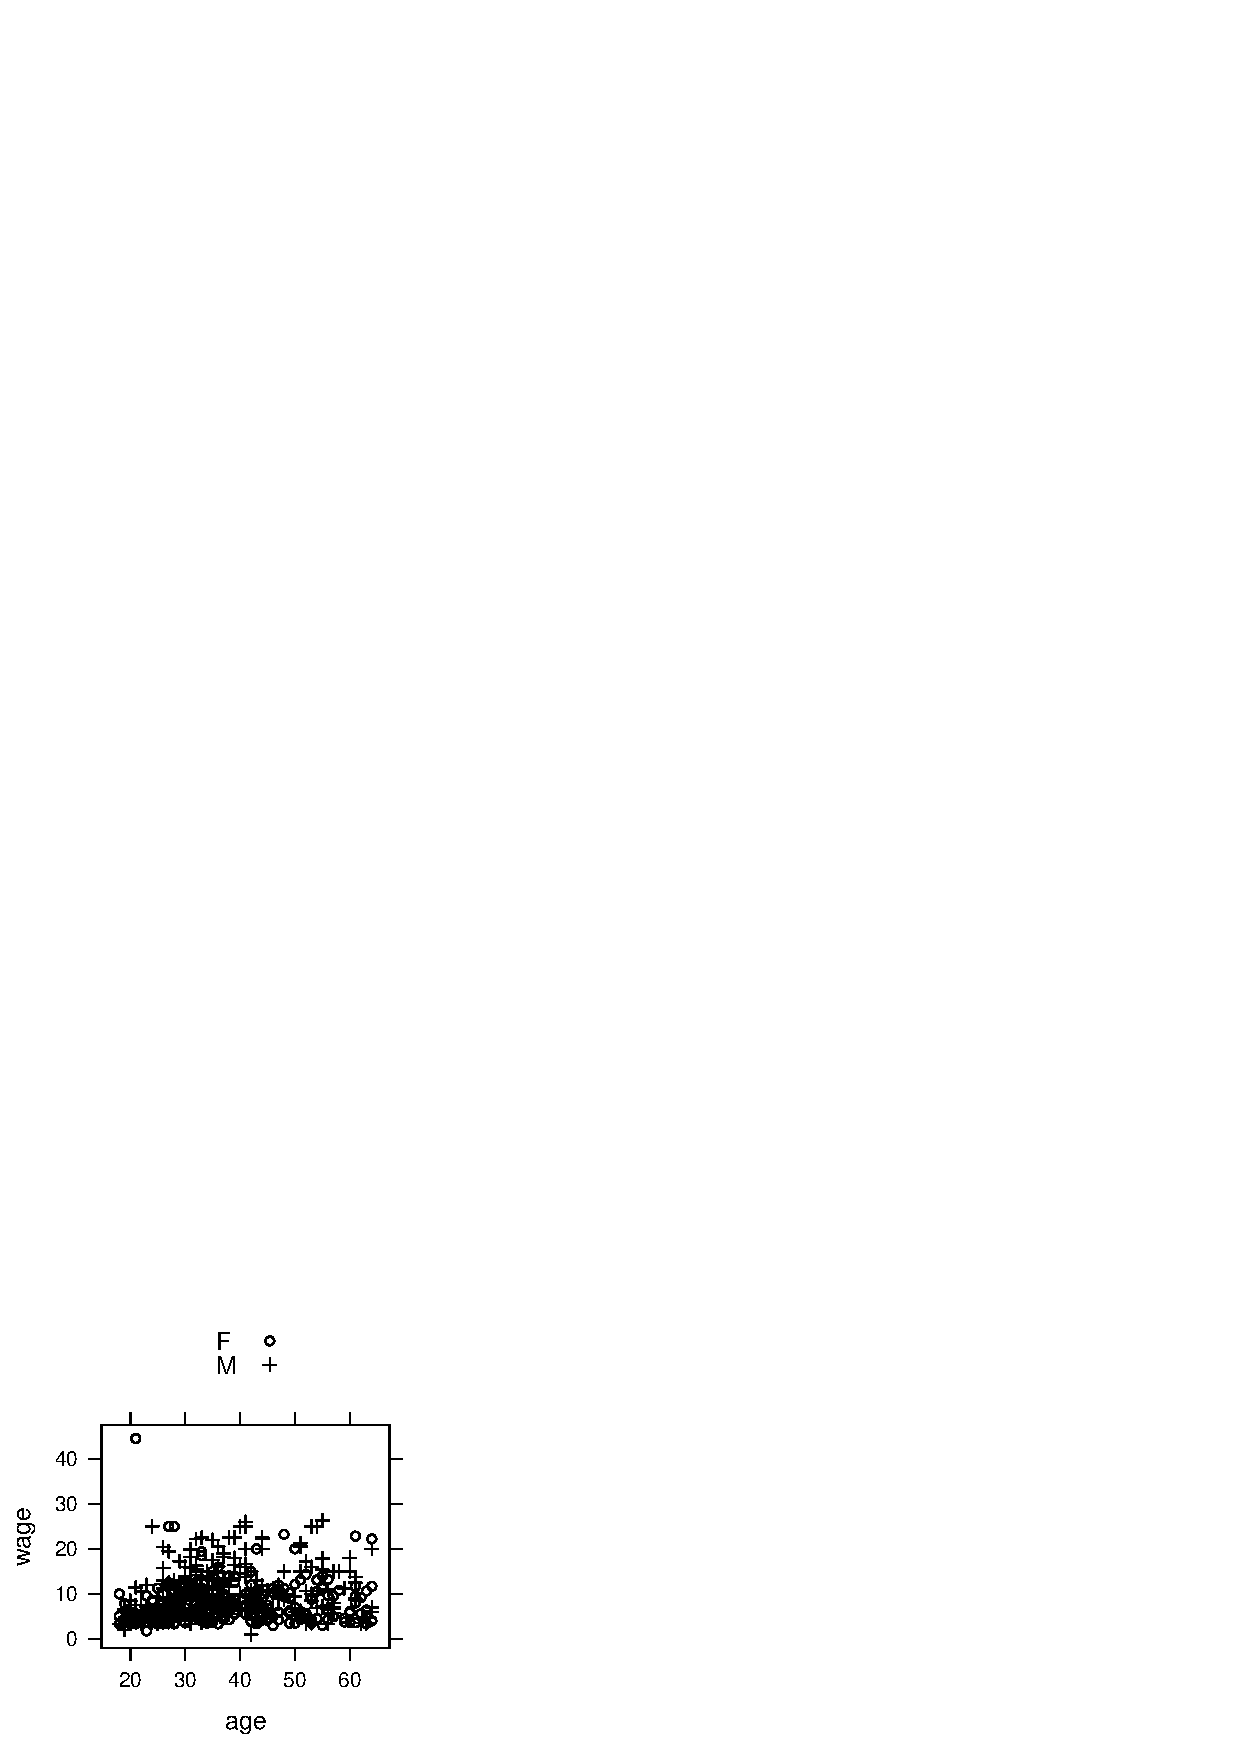
\includegraphics{Figures/language-scatter4}
%\noindent\graphicsfile[width=2.5in]{scatter4.pdf}

\item[Splitting the plot] into the groups defined by the additional
  explanatory variable.  This is done by including the additional
  variable in the model formula using a \code{|} separator.  For
  example:)
\begin{Schunk}
\begin{Sinput}
> xyplot(wage ~ age | sex, data=cps)
\end{Sinput}
\end{Schunk}
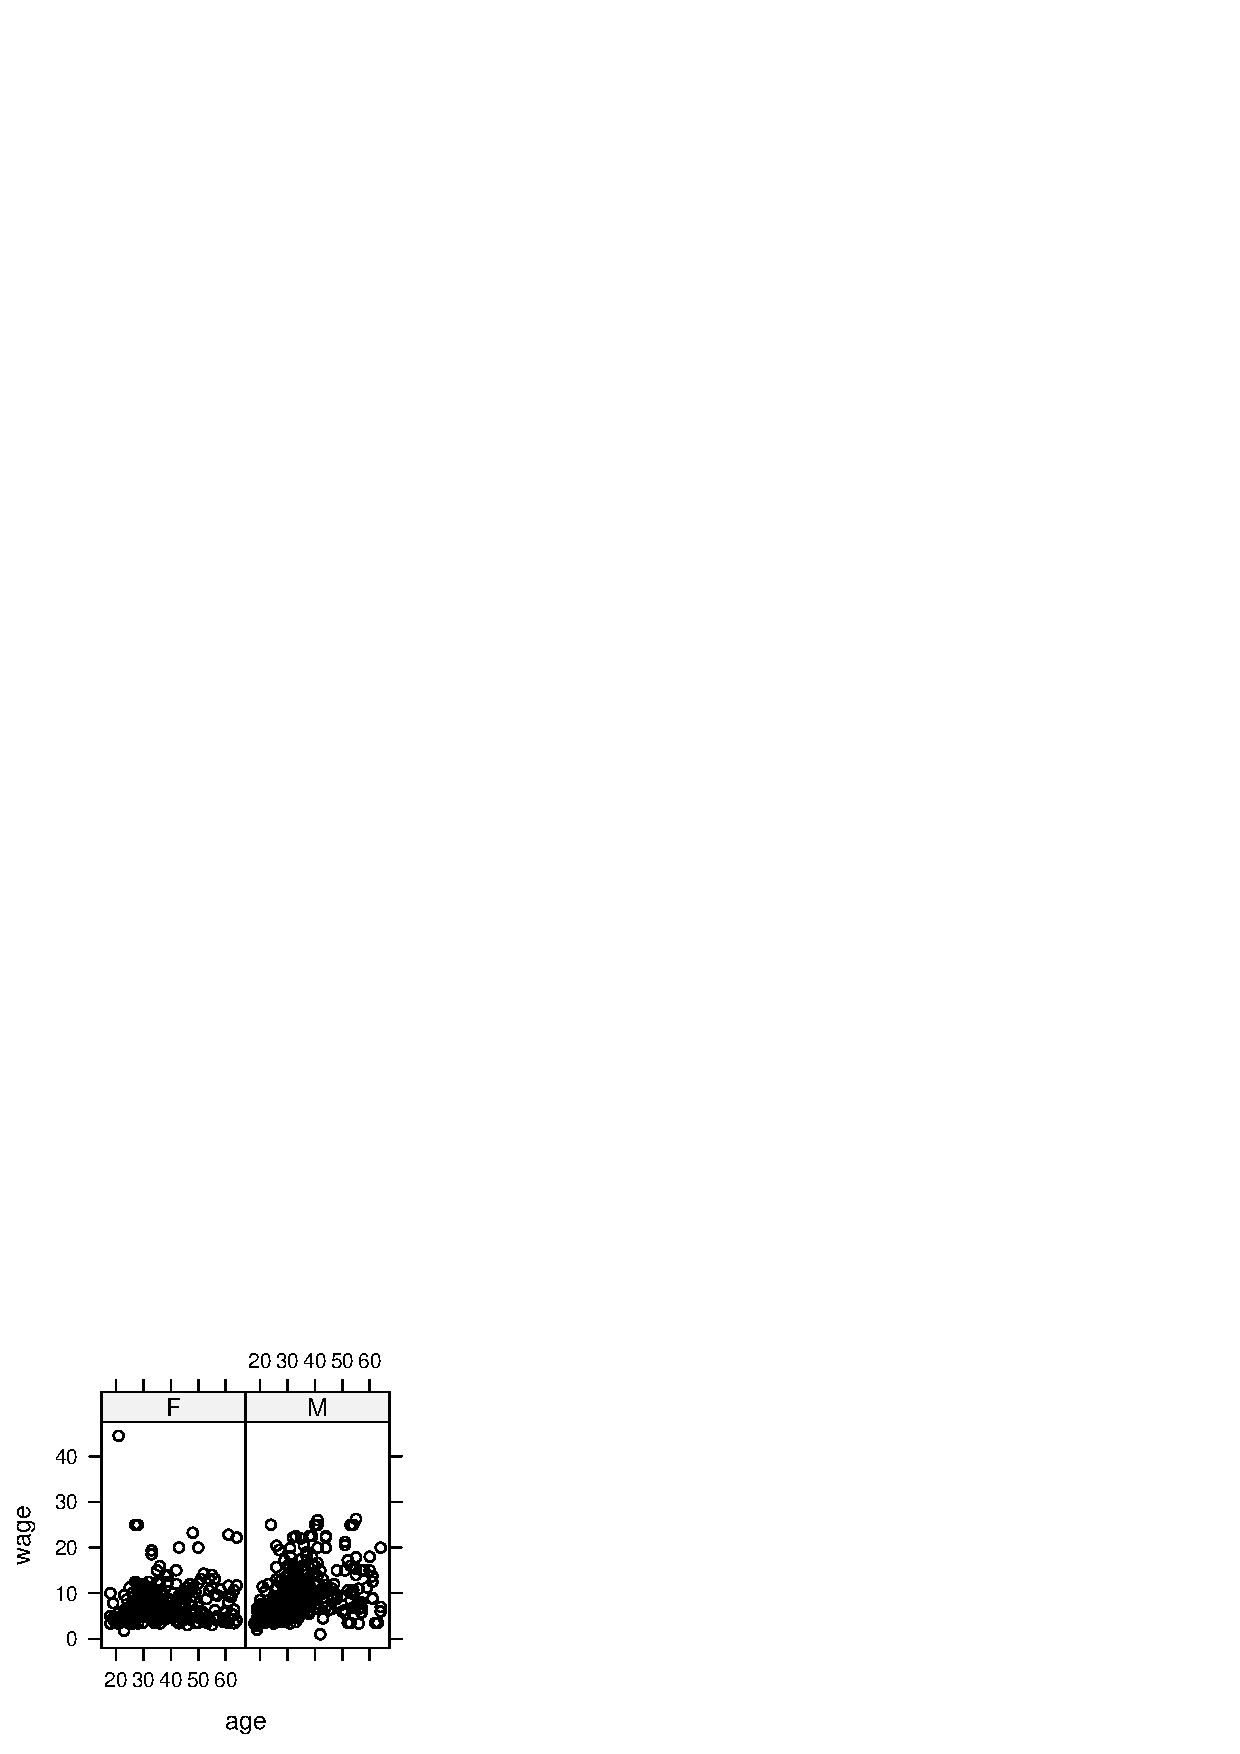
\includegraphics{Figures/language-scatter3}
%\noindent\graphicsfile[width=2.5in]{scatter3.pdf}

\end{description}



\subsection{Fitting Models and Finding Model Values}

The \code{lm} operator (short for ``Linear Model'') will translate a
model design into fitted model values. 
\index{C}{fitting!lm@\texttt{lm} operator}
\index{C}{model fitting!lm@\texttt{lm} operator}
\index{P}{lm@\texttt{lm}}
\index{P}{Modeling!lm@\texttt{lm}}
It does this by ``fitting''
the model to data, a process that will be explained in later
chapters.  For now, focus on how to use \code{lm} to compute the
fitted model values.

The \code{lm} operator uses the same model language as in the
book. To illustrate, consider the world-record swim-times data :
\begin{Schunk}
\begin{Sinput}
> swim = fetchData("swim100m.csv")
\end{Sinput}
\end{Schunk}

To construct the model \model{\VN{time}}{1} for the swim data:
\begin{Schunk}
\begin{Sinput}
> mod1 = lm( time ~ 1, data=swim)
\end{Sinput}
\end{Schunk}
Here the model has been given a name, \code{mod1}, so that you can
refer to it later.  You can use any name you like, so long as it is valid in R.

\datasetSwimming


\index{C}{fitted model values!computing}
\index{P}{fitted@\texttt{fitted}}
\index{P}{Modeling!fitted@\texttt{fitted}}

Once the model has been constructed, the fitted values can be found
using the \code{fitted} operator:
\begin{Schunk}
\begin{Sinput}
> fitted(mod1)
\end{Sinput}
\end{Schunk}
\begin{Schunk}
\begin{Soutput}
   1    2    3    4    5    6    7    8    9   10   11   12 
59.9 59.9 59.9 59.9 59.9 59.9 59.9 59.9 59.9 59.9 59.9 59.9 
... for 62 cases altogether ...
\end{Soutput}
\end{Schunk}

There is an individual fitted model value for each case.
Of course, in this model all the model values are exactly the same
since the model \model{\VN{time}}{1} treats all the cases as
exactly the same.

In later chapters you'll see how to analyze the model values, make 
predictions from the model, and
assess the contribution of each model term.  For now, just look at the model
values by plotting them out along with the data used.  I'll plot out
both the data values and the model values versus \VN{year} just to
emphasize that the model values are the same for every case:

\begin{Schunk}
\begin{Sinput}
> xyplot( time + fitted(mod1) ~ year, data=swim)
\end{Sinput}
\end{Schunk}
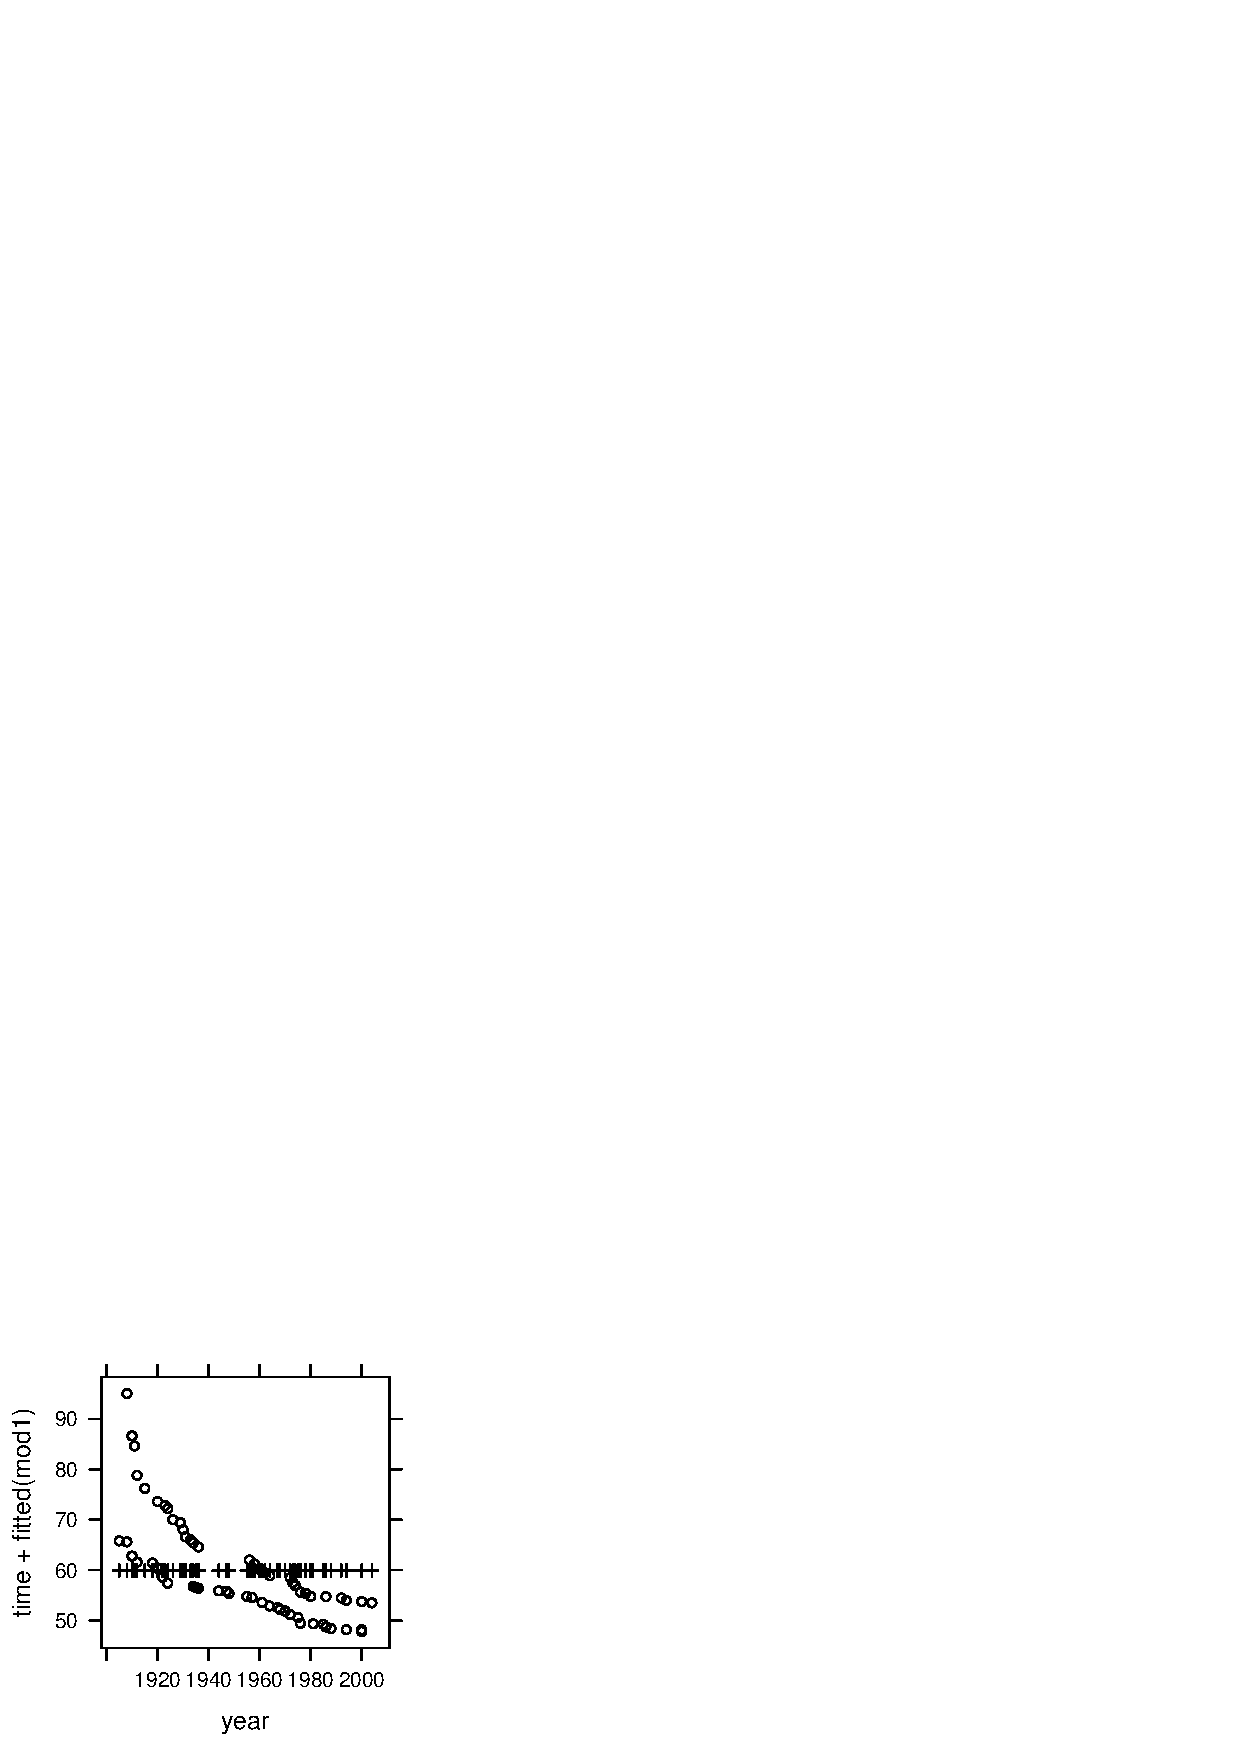
\includegraphics{Figures/language-fitted1}
% \noindent\graphicsfile[width=2.5in]{fitted1.pdf}

Pay careful attention to the syntax used in the above command.  There
are two quantities to the left of the \code{~}.  This is not part of
the modeling language, where there is always a single response
variable.  Instead, it is a kind of shorthand, telling \code{xyplot}
that it should plot out {\em both} of the quantities on the left side
against the quantity on the right side.  Of course, if you wanted to
plot just the model values, without the actual data, you could specify
the formula as \code{fitted(mod1) ~ year}.  

Here are more interesting models:
\begin{Schunk}
\begin{Sinput}
> mod2 = lm( time ~ 1+year, data=swim)
> mod3 = lm( time ~ 1+sex, data=swim)
> mod4 = lm( time ~ 1+sex+year, data=swim)
> mod5 = lm( time ~ 1+year+sex+year:sex, data=swim)
\end{Sinput}
\end{Schunk}

\index{P}{Modeling!a@\texttt{:} and \texttt{*}}

You can, if you like, compare the fitted values from different models
on one plot:
\begin{Schunk}
\begin{Sinput}
> xyplot( fitted(mod5) + fitted(mod3) ~ year, data=swim, 
    auto.key=TRUE)
\end{Sinput}
\end{Schunk}
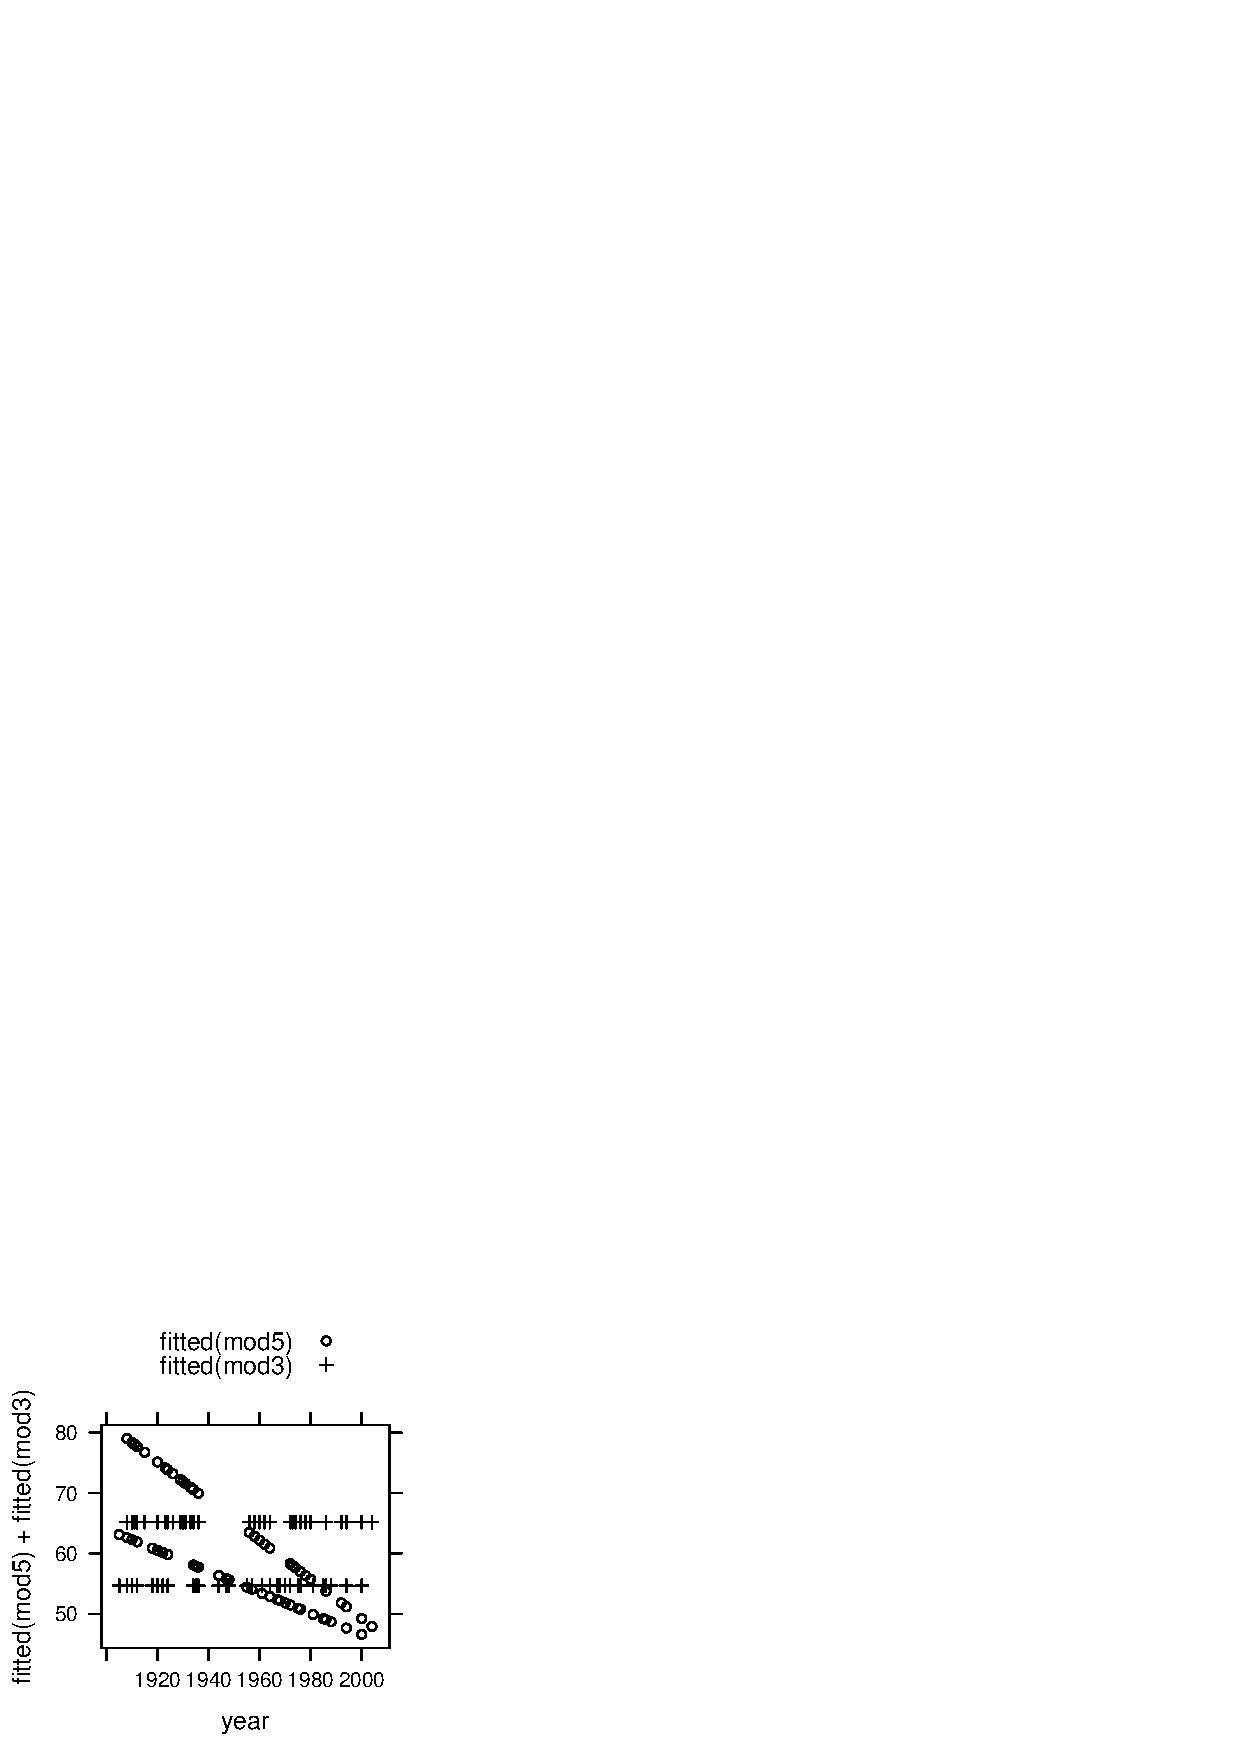
\includegraphics{Figures/language-fitted2}
%\noindent\graphicsfile[width=2.5in]{fitted2.pdf}



\subsubsection{Interactions and Main Effects}

Typically a model that includes an interaction term between two
variables will include the
main terms from those variables too.  As a shorthand for this, the
modeling language has a \code{*} symbol.  So, the formula
\code{time ~ year + sex + year:sex} can also be written 
\code{time ~ year * sex}.

\subsubsection{Transformation Terms}

\index{C}{transformation terms}
\index{P}{I for transformation terms@\texttt{I} for transformation terms}
\index{P}{Modeling!I@\texttt{I} for transformation terms}
Transformation terms such as squares can also be included in the model formula. 
To mark the quantity clearly as a single term, it's best to wrap the
term with \code{I()} as follows:
\begin{Schunk}
\begin{Sinput}
> mod7 = lm( time ~ year + I(year^2) + sex, data=swim)
\end{Sinput}
\end{Schunk}

Another way to accomplish this, for polynomials, is to use the
operator \code{poly} as in the model formula \code{time ~ poly(year,2)+sex}.

Here's a plot of the result:
\begin{Schunk}
\begin{Sinput}
> xyplot( time + fitted(mod7) ~ year, data=swim)
\end{Sinput}
\end{Schunk}
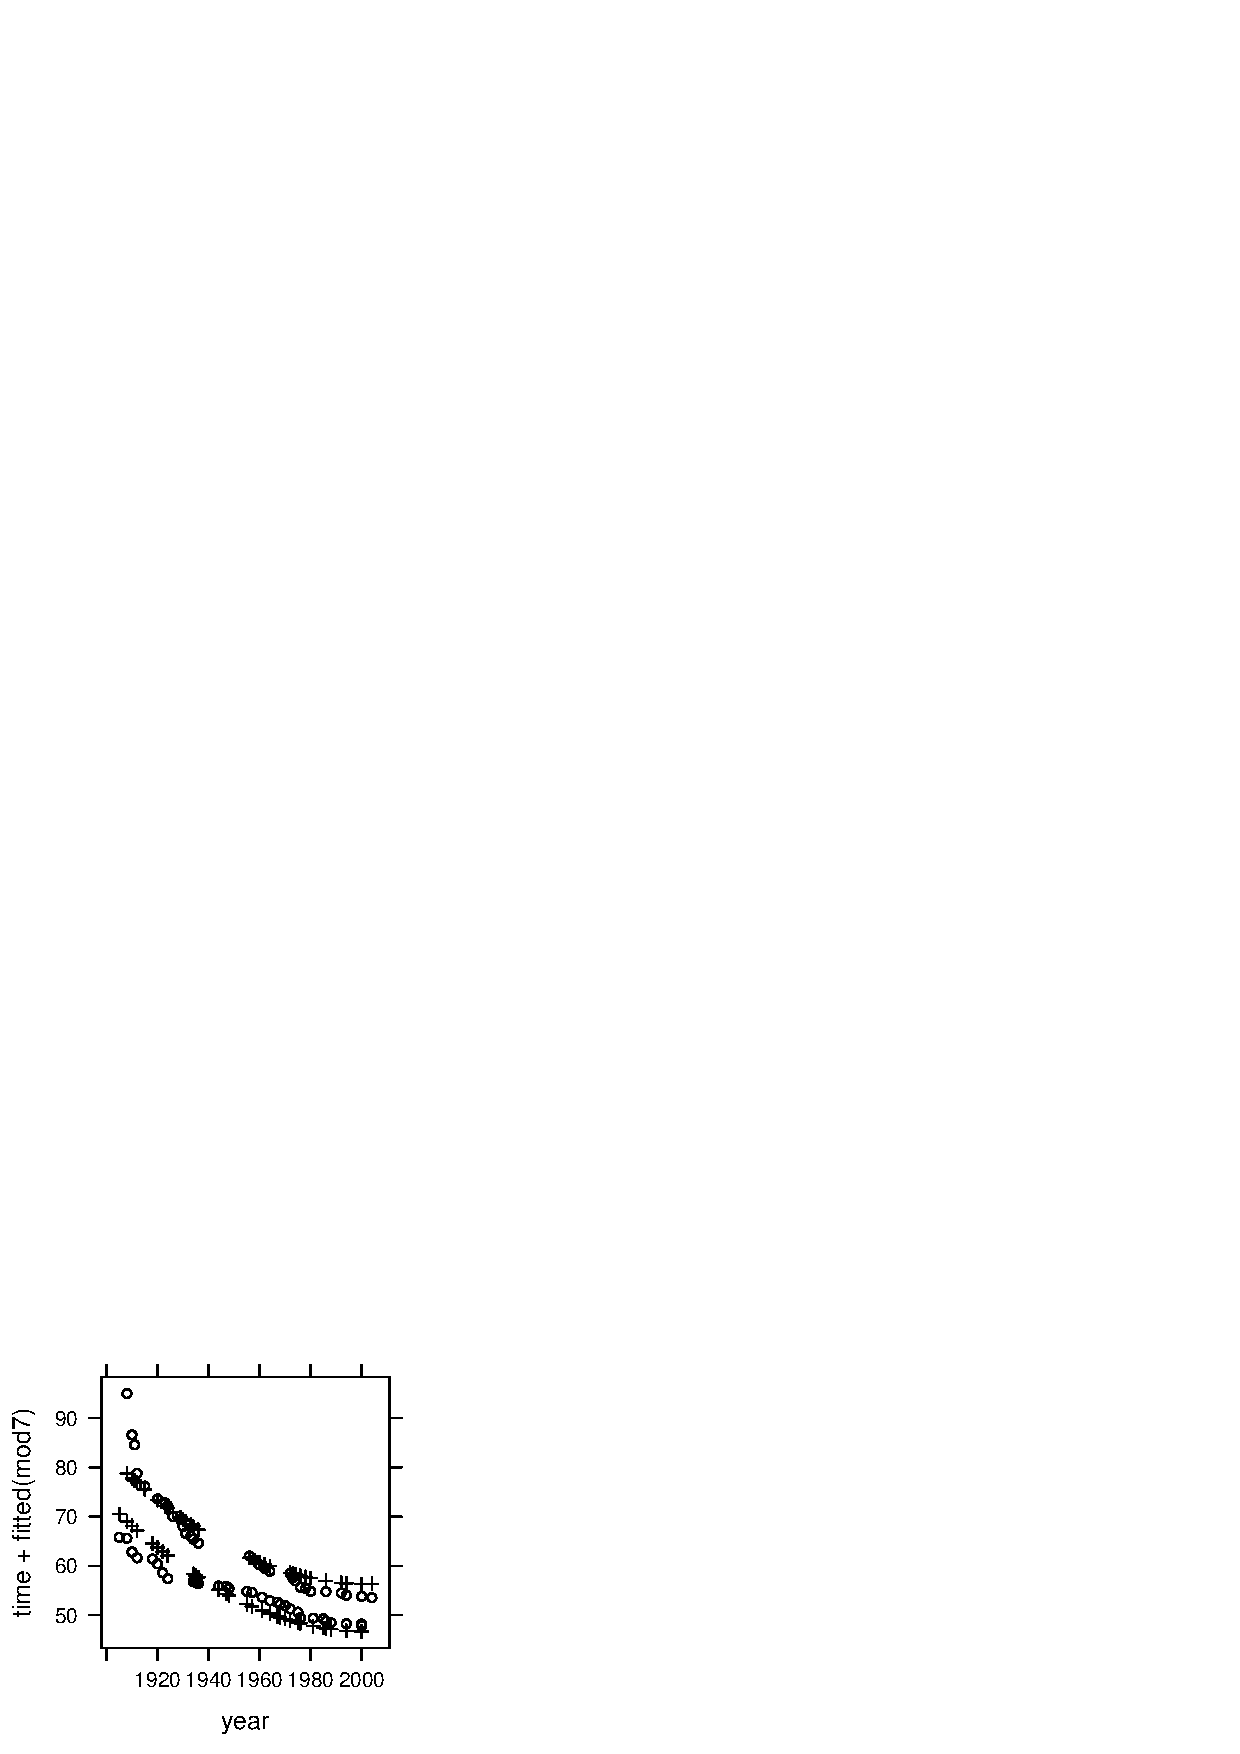
\includegraphics{Figures/language-fitted4}
% \noindent\graphicsfile[width=2.5in]{fitted4.pdf}

